\documentclass[a4paper]{article}
\usepackage[utf8]{inputenc}
\usepackage[spanish, es-tabla, es-noshorthands]{babel}
\usepackage[table,xcdraw]{xcolor}
\usepackage[a4paper, footnotesep = 1cm, width=22cm, top=2.5cm, height=25cm, textwidth=20cm, textheight=25cm]{geometry}
%\geometry{showframe}

\usepackage{tikz}
\usepackage{amsmath}
\usepackage{amsfonts}
\usepackage{amssymb}
\usepackage{float}
\usepackage{graphicx}
\usepackage{caption}
\usepackage{subcaption}
\usepackage{multicol}
\usepackage{multirow}
\usepackage{wrapfig}
\setlength{\doublerulesep}{\arrayrulewidth}
\usepackage{booktabs}

\usepackage{hyperref}
\hypersetup{
    colorlinks=true,
    linkcolor=blue,
    filecolor=magenta,      
    urlcolor=blue,
    citecolor=blue,    
}

\newcommand{\note}[1]{
	\begin{center}
		\huge{ \textcolor{red}{#1} }
	\end{center}
}

\setcounter{topnumber}{2}
\setcounter{bottomnumber}{2}
\setcounter{totalnumber}{4}
\renewcommand{\topfraction}{0.85}
\renewcommand{\bottomfraction}{0.85}
\renewcommand{\textfraction}{0.15}
\renewcommand{\floatpagefraction}{0.8}
\renewcommand{\textfraction}{0.1}
\setlength{\floatsep}{5pt plus 2pt minus 2pt}
\setlength{\textfloatsep}{5pt plus 2pt minus 2pt}
\setlength{\intextsep}{5pt plus 2pt minus 2pt}

\newcommand{\quotes}[1]{``#1''}
\usepackage{array}
\newcolumntype{C}[1]{>{\centering\let\newline\\\arraybackslash\hspace{0pt}}m{#1}}
\usepackage[american]{circuitikz}
\usetikzlibrary{calc}
\usepackage{fancyhdr}
\usepackage{units} 

\graphicspath{{../Ejercicio-1/}{../Ejercicio-2/}{../Ejercicio-3/}{../Ejercicio-4/}{../ParteI/}{../ParteII/}{../ParteIII/}{../ParteIV/}}

\pagestyle{fancy}
\fancyhf{}
\lhead{22.14 - Electrónica IV}
\rhead{Mechoulam, Lambertucci, Londero}
\rfoot{Página \thepage}


\begin{document}

\subsection{Introducción}

Dada una fuente Boost con una tensión de entrada $12 \ V$ y frecuencia de switching de $60 \ kHz$, se buscó determinar el Duty Cicle necesario tal que la tensión de salida sea de $24 \ V$ y tenga una variación del $5\%$. Cabe notar que esta fuente Boost es una no ideal ya que se considera la resistencia de la bobina $R_4 = 2 \ \Omega$.

\begin{figure}[H]
	\centering
	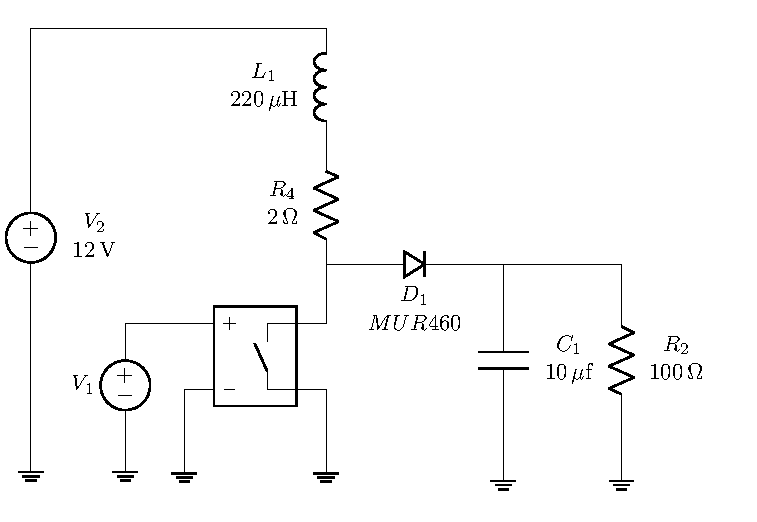
\includegraphics[width=0.7\linewidth, page=1]{ImagenesEjercicio-2/CircuitsEj2}
	\caption{Circuito de fuente Boost con llave ideal.}
	\label{fig:ej2:circuito}
\end{figure}

\subsection{Calculo del Duty Cicle}

%Utilizando la transferencia de la fuente Boost ideal, es decir sin $R_4$, se puede obtener el Duty Cicle deseado:
%
%\begin{align*}
%V_o &= \frac{V_2}{1 - d}	\\
%1 - d &= \frac{V_2}{V_o} = \frac{12 \ V}{24 \ V} \\
%d &= 0.5
%\end{align*}

\end{document}